\chapter{\textit{Scheduling} en motores de búsqueda}
\label{cap:eda}

Los sistemas de recuperación de la información como los motores de búsqueda, no solo se preocupan de la calidad de los resultados de las búsquedas (efectividad), sino que también de la velocidad con la que los resultados son obtenidos (eficiencia). Existen varias estrategias para mejorar la velocidad en la obtención de los resultados, una de ellas muy utilizada es el \textit{caching}. Consiste en guardar en memoria de acceso rápido (memoria caché) datos temporales, que luego pueden ser sobrescrito. Una opción es hacer \textit{caching} de los resultados de las búsquedas, de esta forma cuando una \textit{query} es encontrada en caché el motor de búsqueda puede generar la respuesta rápidamente, reduciendo los tiempos de calculos considerablemente. Otra opción es, guardar en caché la intersección de las listas invertidas de pares comunes de términos que llegan al motor de búsqueda. Por ejemplo, si llega al sistema una consulta con los términos ('casa', 'árbol', 'perro'), se puede guardar en caché la intersección de las listas de 'casa' y 'árbol', para luego reutilizar esta información en otras \textit{queries} que lleguen en el futuro. Para ver más técnicas de \textit{caching} y ver el detalle de las técnicas mencionadas, ver \citep{Buttcher:2010}.

Otra estrategia para acelerar el proceso de resolución de \textit{queries} que llegan al sistema es el uso de algoritmos de planificación (scheduling). Un algoritmo de \textit{scheduling} es el proceso en el cual se cambia el orden en que llegan las \textit{queries} al motor de búsqueda con el objetivo de mejorar la eficiencia. 

Existen dos clases de algoritmos de \textit{scheduling}, estáticos y dinámicos. Los estáticos son aquellos en que se conoce el conjunto completo de tareas y las características de cada una de ellas, como por ejemplo, el tiempo de procesamiento. Los algoritmos de \textit{scheduling} dinámicos son aquellos en que no se conoce las tareas que llegarán en el futuro, también se desconoce el momento en que éstas llegarán. La filosofía de los algoritmos de \textit{scheduling} dinámicos es ajustarse a los cambios que pueden haber en el sistema.

En el contexto del presente trabajo de tesis, el objetivo de hacer \textit{scheduling} es minimizar el tiempo en que las \textit{queries} son procesadas por un motor de búsqueda. Los motores de búsqueda como \textit{Google}\footnote{http://www.google.com} o \textit{Yahoo!}\footnote{http://www.yahoo.com} trabajan en un contexto \textit{online}. Esto significa que cuando las \textit{queries} llegan al sistema (una a una), éste está obligado a tomar una decisión para planificarla sin saber cuáles \textit{queries} llegarán en un momento posterior. A esto se le conoce como algoritmo de \textit{scheduling online} \citep{Albers:2003, Borodin:1998}.

Los sistemas IR a gran escala despliegan una arquitectura distribuída \citep{Dean:2009}, en donde el índice invertido está particionado a lo largo de servidores (\textit{shard servers}), los cuales están encargados de procesar las \textit{queries} que llegan al sistema. Es fácil notar que resolver una \textit{query} con varios \textit{shard servers} mejoraría la eficiencia. Ahora bien, para asegurar un alto rendimiento (\textit{throughput}) del sistema, cada uno de los \textit{shard servers} posee réplicas, de esta forma, más \textit{queries} pueden ser procesadas en paralelo en copias idénticas del mismo \textit{shard server}. Esto implica que el tiempo de espera de las \textit{queries} que vienen llegando al sistema se reduce. 

Como en un sistema con arquitectura como el de la Figura \ref{fig:sistemaIR}, una \textit{query} puede ser procesada por varios \textit{shard servers}, el \textit{broker} debe escoger la réplica más apropiada para procesar la parte de la \textit{query} asignada al \textit{shard server}, con el objetivo de reducir el tiempo de espera de ésta. El \textit{broker} podría seleccionar el \textit{shard server} con el menor número de \textit{queries} en la cola, sin embargo, este no es un parámetro adecuado, ya que el tiempo de respuesta de las \textit{queries} puede variar considerablemente, especialmente si se usa poda dinámica \citep{Broder:2003, Moffat:1996}. 

\begin{figure}[tp]
\centering
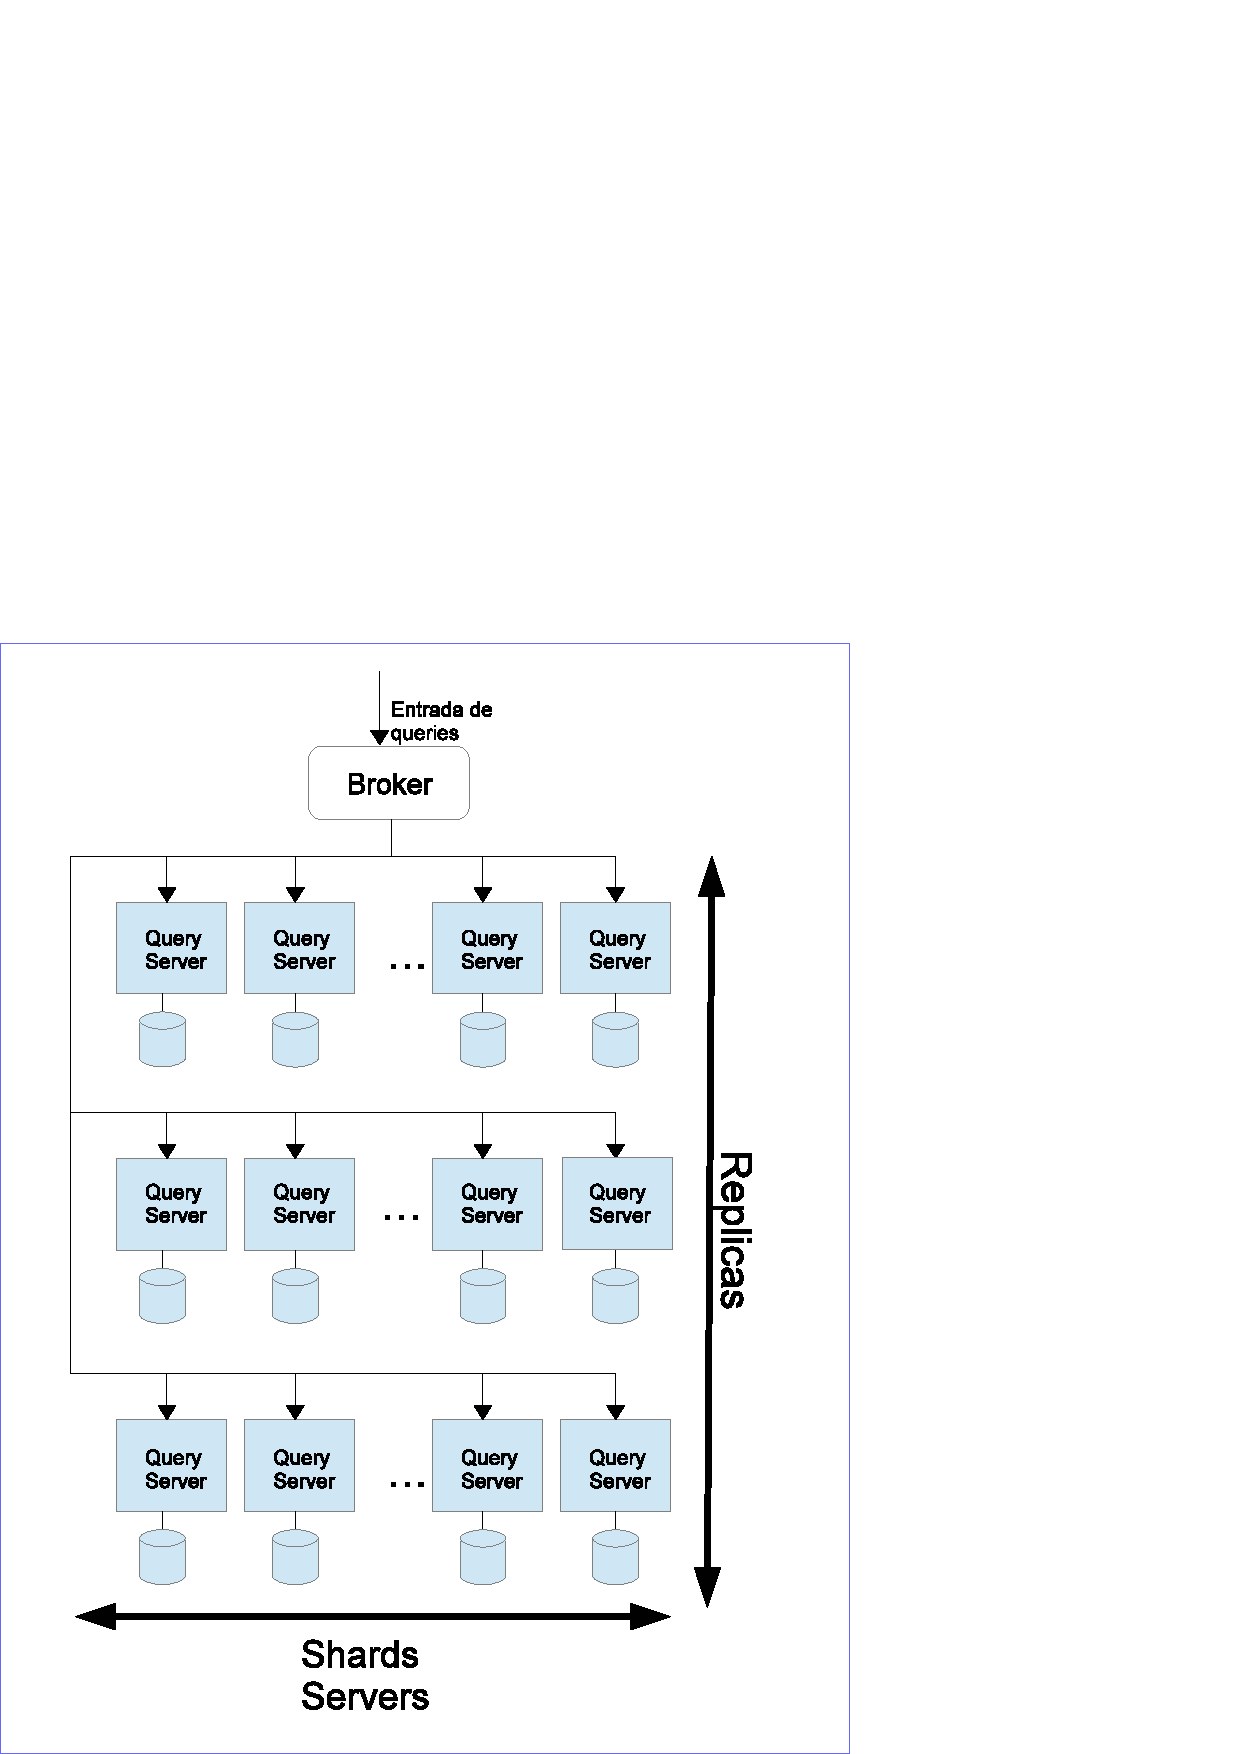
\includegraphics[scale=.75]{images/sistemaIR.png}
\caption{Arquitectura de un sistema de recuperación de la información con réplicas}
\label{fig:sistemaIR}
\end{figure}


\section{Trabajo relacionado}
\label{scheduling:tr}
El estudio \citep{Broccolo:2013} analiza métodos de \textit{dropping} y \textit{stopping} para el procesamiento de \textit{queries} bajo altas carga de trabajo en un sistema distribuído donde existen múltiples servidores en el que cada uno resuelve una parte de la \textit{query} para luego enviar las consultas al \textit{broker} y éste hace el \textit{merge} de los resultados de acuerdo al \textit{score} de los documentos. Se define un tiempo \textit{T}, en el que la suma de el tiempo de espera de la \textit{query} para ser procesada ($t_{w}$) y el tiempo de procesamiento de la misma ($t_{p}$) deben ser menor a \textit{T}. Si es que se sobrepasa este tiempo, se tienen dos opciones (1) la \textit{query} es desechada y se envía al \textit{broker} una lista vacía, (2) se detiene el procesamiento de la \textit{query} y se envía los resultados parciales hasta el momento. Finalmente se propone un método basado en la predicción de tiempo de respuesta ($\hat{pt}(q)$) de una \textit{query} \citep{Macdonald:2012} de modo que si se cumple $ \hat{pt}(q) \leq T - wt(q) $, entonces la \textit{query} es desechada antes de comenzar a procesarse y se toma la siguiente desde la cola de espera. Notar que en estos métodos existe una pérdida de efectividad, puesto que eventualmente los servidores muchas veces no enviarán sus mejores documentos al \textit{broker}, esto implica que el \textit{broker} responderá al usuario un conjunto de K documento que no necesariamente son los mejores dentro del corpus completo.

En \citep{Freire:2012} se estudia el impacto que tiene la técnica de predicción de tiempos de respuestas para \textit{queries}, \citep{Tonellotto:2011} en sistemas de recuperación de la información con réplicas. En este estudio, se llega a la conclusión que usando una buena predicción, se puede reducir el tiempo que la \textit{query} tiene que esperar para ser procesada ($t_{w}$), y también se puede reducir el tiempo total requerido para procesar el conjunto (\textit{log}) completo de \textit{queries} (\textit{completion time}). En \citep{Freire:2013}, se propone un modelo híbrido de \textit{scheduling} de \textit{queries} a través de réplicas, en el que cuando el sistema se encuentre bajo altas cargas de trabajo, se utilice política de \textit{scheduling} basada en la predicción de tiempo de respuesta de las \textit{queries} \citep{Macdonald:2012} y cuando el sistema se encuentre con una baja carga de trabajo, se utilice una politica de \textit{scheduling} sencilla y de menor costo como \textit{Round Robin}.


\section{Predicción del tiempo de respuesta a \textit{queries} en un motor de búsqueda}
\label{scheduling:ptrq}
Conocer de antemano la eficiencia de una \textit{query} es una ventaja importante para usar técnicas efectivas de \textit{scheduling} de \textit{queries} en motores de búsqueda. Existen estudios en los cuales la eficiencia es inferida usando \textit{clarity score} \citep{Cronen-Townsend:2002}, que es una forma para evaluar la pérdida de ambigüedad de una query con respecto a la colección. En \citep{He:2004} se propone un conjunto de predictores para la eficiencia de cada \textit{query}. Técnicas de aprendizaje de máquina también han sido estudiadas para predecir la eficiencia de \textit{queries} \citep{Si:2002}. Todos los estudios mencionados anteriormente se han centrado en la efectividad para ser predicciones. La eficiencia también ha sido utilizada para predecir el tiempo de respuesta de una query, identificando las razones por las que ésta puede ser resuelta ineficientemente y evaluando estos factores para predecir el comportamiento de futuras queries \citep{Tonellotto:2011}.

En el predictor propuesto en \citep{Macdonald:2012} está basado en estadísticos  disponibles de los términos de la query. 

\begin{tabular}{|l|}
\hline 
Estadístico del término s(t) \\ 
\hline 
1. Media aritmética del score \\ 
\hline 
2. Media geométrica del score \\ 
\hline 
3. Media armonica del score \\ 
\hline 
4. Puntaje máximo \\ 
\hline 
5. Varianza de puntaje \\ 
\hline 
6.  \\ 
\hline 
Agregadores \\ 
\hline 
Máximo \\ 
\hline 
Varianza \\ 
\hline 
Suma \\ 
\hline 
\end{tabular} 


Este predictor está evaluado comparado con 10.000 queries == individual and combinated


\section{Wand \textit{multi-threading}}
\label{scheduling:wm}

\subsection{Wand con heaps locales}
\label{scheduling:whl}
...

\subsection{Wand con heap compartido}
\label{scheduling:whc}
...


\subsection{Evaluación de los esquemas}
\label{scheduling:we}
...



\section{Wand \textit{multi-threading}}
\label{scheduling:wm}


\section{Estrategias de \textit{scheuling}}
\label{scheduling:es}

\subsection{FR}
\label{scheduling:fr}

\subsection{Times}
\label{scheduling:times}

\subsection{TimesRanges}
\label{scheduling:timesranges}







